% This file was converted to LaTeX by Writer2LaTeX ver. 1.0.2
% see http://writer2latex.sourceforge.net for more info
\documentclass[twoside,letterpaper]{article}
\usepackage[latin1]{inputenc}
\usepackage[T1]{fontenc}
\usepackage[english]{babel}
\usepackage{amsmath}
\usepackage{amssymb,amsfonts,textcomp}
\usepackage{color}
\usepackage{array}
\usepackage{longtable}
\usepackage{hhline}
\usepackage{hyperref}
\usepackage{datetime}
\hypersetup{pdftex, colorlinks=true, linkcolor=blue, citecolor=blue, filecolor=blue, urlcolor=blue, pdftitle=SOFTWARE DESIGN SPECIFICATION, pdfauthor=Serta\c{c} Karahoda, pdfsubject=, pdfkeywords=}
\usepackage[pdftex]{graphicx}
% Outline numbering
\setcounter{secnumdepth}{5}
\renewcommand\thesection{\arabic{section}}
\renewcommand\thesubsection{\arabic{section}.\arabic{subsection}}
\renewcommand\thesubsubsection{\arabic{section}.\arabic{subsection}.\arabic{subsubsection}}
\renewcommand\theparagraph{\arabic{section}.\arabic{subsection}.\arabic{subsubsection}.\arabic{paragraph}}
\renewcommand\thesubparagraph{\arabic{section}.\arabic{subsection}.\arabic{subsubsection}.\arabic{paragraph}.\arabic{subparagraph}}
\makeatletter
\newcommand\arraybslash{\let\\\@arraycr}
\makeatother
% List styles
\newcommand\liststyleWWviiiNumii{%
\renewcommand\theenumi{\arabic{enumi}}
\renewcommand\theenumii{\arabic{enumii}}
\renewcommand\theenumiii{\arabic{enumiii}}
\renewcommand\theenumiv{\arabic{enumiv}}
\renewcommand\labelenumi{\theenumi)}
\renewcommand\labelenumii{\theenumii.}
\renewcommand\labelenumiii{\theenumiii.}
\renewcommand\labelenumiv{\theenumiv.}
}
% Page layout (geometry)
\setlength\voffset{-1in}
\setlength\hoffset{-1in}
\setlength\topmargin{0.5in}
\setlength\oddsidemargin{1in}
\setlength\evensidemargin{1in}
\setlength\textheight{8.278in}
\setlength\textwidth{6.5in}
\setlength\footskip{0.561in}
\setlength\headheight{0.5in}
\setlength\headsep{0.461in}
% Footnote rule
\setlength{\skip\footins}{0.0469in}
\renewcommand\footnoterule{\vspace*{-0.0071in}\setlength\leftskip{0pt}\setlength\rightskip{0pt plus 1fil}\noindent\textcolor{black}{\rule{0.25\columnwidth}{0.0071in}}\vspace*{0.0398in}}
% Pages styles
\makeatletter
\newcommand\ps@Standard{
  \renewcommand\@oddhead{\selectlanguage{english}\rmfamily\color{black} Sabanc{\i} University CS Department Instructional Use\hfill \hfill Scheduler}
  \renewcommand\@evenhead{\@oddhead}
  \renewcommand\@oddfoot{\foreignlanguage{english}{\textcolor{black}{\centerline{\thepage{}}}}}
  \renewcommand\@evenfoot{\@oddfoot}
  \renewcommand\thepage{\arabic{page}}
}
\newcommand\ps@Preface{
  \pagenumbering{Roman}
  \renewcommand\@oddhead{\selectlanguage{english}\rmfamily\color{black} Sabanc{\i} University CS Department Instructional Use\hfill \hfill Scheduler}
  \renewcommand\@evenhead{\@oddhead}
  \renewcommand\@oddfoot{\foreignlanguage{english}{\textcolor{black}{\centerline{\thepage{}}}}}
  \renewcommand\@evenfoot{\@oddfoot}
  \renewcommand\thepage{\roman{page}}
}
\newcommand\ps@Appendix{
  \renewcommand\@oddhead{}
  \renewcommand\@evenhead{\@oddhead}
  \renewcommand\@oddfoot{}
  \renewcommand\@evenfoot{\@oddfoot}
  \renewcommand\thepage{\arabic{page}}
}
\makeatother
\pagestyle{Standard}
\setlength\tabcolsep{1mm}
\renewcommand\arraystretch{1.3}
\title{SOFTWARE DESIGN SPECIFICATION}
\author{Serta\c{c} Karahoda}
\date{\currenttime}
\begin{document}
\clearpage\setcounter{page}{1}\pagestyle{Standard}
\thispagestyle{Preface}

\vspace*{1.5in}
{\centering\selectlanguage{english}\bfseries\color{black}
 SOFTWARE DESIGN SPECIFICATION (SDS) FOR 
\par}

\bigskip

{\centering\selectlanguage{english}\bfseries\color{black}
SCHEDULER
\par}


\bigskip


\bigskip


\bigskip


\bigskip

{\centering\selectlanguage{english}\bfseries\color{black}
Version 1.0
\par}

{\centering\selectlanguage{english}\bfseries\color{black}
16 March 2015
\par}


\bigskip


\bigskip

{\centering\selectlanguage{english}\bfseries\color{black}
Prepared for:
\par}

{\centering\selectlanguage{english}\bfseries\color{black}
Ramin Armanfar <raminarmanfar@sabanciuniv.edu>

\par}


\bigskip


\bigskip

{\centering\selectlanguage{english}\bfseries\color{black}
Prepared by:
\par}

{\centering\selectlanguage{english}\bfseries\color{black}
Berk \c{C}iri\c{s}ci <berkcirisci@sabanciuniv.edu>

Elif Meri\c{c} <elifmeric@sabanciuniv.edu>

Pamir Mundt <pamirmundt@sabanciuniv.edu>

Serta\c{c} Karahoda <skarahoda@sabanciuniv.edu>

Yavuz Selim Emir <yavuzselim@sabanciuniv.edu>
\par}

\clearpage{\centering\selectlanguage{english}\bfseries\color{black}
SDS
\par}

{\centering\selectlanguage{english}\bfseries\color{black}
RECORD OF CHANGES (Change History)
\par}

\begin{flushleft}
\begin{longtable}{|m{0.47685984in}|m{1.2418196in}|m{1.3587599in}|m{0.23375985in}|m{2.0462599in}|m{0.9337598in}|}
\hline
~

\centering \selectlanguage{english}\color{black} Change number &
~

\centering \selectlanguage{english}\color{black} Date completed &
~

\centering \selectlanguage{english}\color{black} Location of change
(e.g., page or figure \#) &
\centering \selectlanguage{english}\bfseries\color{black} A\newline
M\newline
D &
~

\centering \selectlanguage{english}\color{black} Brief description of
change &
~

\centering\arraybslash \selectlanguage{english}\color{black} Author
\\\hline
\endhead
\centering{0}
 &
\centering{9 April 2015}
 &
All
 &
\centering{A}
 &
\raggedright{The document created}
 &
 Serta\c{c}
 \\\hline
 \centering{1}
 &
\centering{12 April 2015}
 &
Section \ref{sec:intro}, \ref{sec:overview}
 &
\centering{M}
 &
 \raggedright{Introduction and System Overview added}
 &
 Berk
 \\\hline
  \centering{2}
 &
\centering{18 April 2015}
 &
Section \ref{sec:description}
 &
\centering{M}
 &
 \raggedright{Detailed Descriptions of components are added}
 &
 Berk, Serta\c{c}
 \\\hline
 \centering{3}
 &
\centering{18 April 2015}
 &
Section \ref{sec:considerations}
 &
\centering{M}
 &
 \raggedright{Design Considerations added}
 &
 Yavuz
 \\\hline
  \centering{4}
 &
\centering{24 April 2015}
 &
Section \ref{sec:considerations}, \ref{sec:architecture}
 &
\centering{M}
 &
 \raggedright{Minor revisions}
 &
Serta\c{c}, Yavuz
 \\\hline
\end{longtable}
\end{flushleft}
{\selectlanguage{english}\color{black}
A - ADDED \ M - MODIFIED \ D -- DELETED}

\clearpage{\centering\selectlanguage{english}\bfseries\color{black}
SCHEDULER
\par}

{\centering\selectlanguage{english}\bfseries\color{black}
TABLE OF CONTENTS
\par}

\setcounter{tocdepth}{9}
\renewcommand\contentsname{}
\tableofcontents

\bigskip

\bigskip
\clearpage\setcounter{page}{1}\pagestyle{Standard}
\section{INTRODUCTION}
\label{sec:intro}

\subsection{IDENTIFICATION}

This document is the software design document of the program called "Scheduler". \ This document is designed for Ramin Armanfar and all developers who are working in the project. \  This a new project effort, so the version under development is Version 1.0.

\subsection{DOCUMENT PURPOSE, SCOPE, AND INTENDED AUDIENCE}

\subsubsection{Document Purpose}

This document will describe the architect of our system and provide a brief summary for the specifications of software design.

\subsubsection{Document Scope}
The scope of this document is to inform our customer about the architect and the design of our system and inform him about the details of our software.

\subsubsection{Intended Audience for Document}

The intended audience of this document originally will be our customer, Ramin Armanfar and the workers of this project but as we released our document on web environment, anyone who are interested with the project can read our document.


\subsection{DEFINITIONS, ACRONYMS, AND ABBREVIATIONS}


\begin{flushleft}
\begin{longtable}{|m{1.3587599in}|m{5.00806in}|}
\hline
\centering \selectlanguage{english}\bfseries\color{black} Term or
Acronym &
\centering\arraybslash \selectlanguage{english}\bfseries\color{black}
Definition\\\hline
\endhead
Architect &
The person, team, or organization responsible for systems
architecture.
\\\hline
Architectural View &
A representation of a whole system from the perspective of a related set
of concerns.
\\\hline
Architecture &
The fundamental organization of a system embodied in its components, their
relationships to each other, and to the environment, and the principles
guiding its design and evolution.
\\\hline
Design View &
A subset of design entity attribute information that is specifically
suited to the needs of a software project activity.
\\\hline
SDS &
Software Design Specification
\\\hline
Software Design Specification &
A representation of a software system created to facilitate analysis,
planning, implementation, and decision making, A blueprint or model of
a software system. The SDS is used as the primary medium for
communicating software design information.
\\\hline
SRS &
Software Requirements
Specification
\\\hline
System &
A collection of components organized to accomplish a specific function or
set of functions.
\\\hline
System Stakeholder &
An individual, team, or organization (or classes thereof) with interests
in, or concerns, relative to, a system.
\\\hline
Bannerweb &
A course registration system for Sabanc{\i} University
\\\hline
Cross platform &
Systems that can run on different operating system like Windows, Linux and Mac OS
\\\hline
Java & 
An object oriented, cross platform programming language
\\\hline
JVM & 
Java Virtual Machine
\\\hline
GPL &
GNU General Public License is a free software license, which guarantees end users the freedoms to use, study, share, and modify the software. 
\\\hline
CRN &
Course Reference Number  
\\\hline
JSoup &
 A Java library for working with real-world HTML  
\\\hline
SQLite &
A software library that implements a self-contained, serverless, zero-configuration, transactional SQL database engine.  
\\\hline
Swing &
 a graphical user interface widget toolkit for Java.
\\\hline
\end{longtable}
\end{flushleft}

\smallskip

\subsection{DOCUMENT OVERVIEW}

\noindent
Section \ref{sec:overview} of this document describes the system and software purpose, scope and intended audience of program. \ 
It describes the functionalities of the program and how it will work while user is using the program. 

\bigskip

\noindent
Section \ref{sec:considerations} of this document describes the considerations of design like assumptions, dependencies, goals, general constraints and priorities. \ It will also describe the issues which should be solved before completing the design.

\bigskip

\noindent
Section \ref{sec:architecture} of this document describes the system and software architecture from several viewpoints, including, chosen system architecture and interface, discussions about other alternative designs. \ It will describe why this architecture selected to design after the discussions about alternative system designs.

\bigskip

\noindent
Section \ref{sec:description} provides detailed design descriptions for every component defined in the architectural view(s). 

\clearpage\pagestyle{Standard}
\section{SYSTEM OVERVIEW}
\label{sec:overview}

\subsection{SYSTEM AND SOFTWARE PURPOSE}

The purpose of the system under development is to make course schedule for Sabanc\i{} University students. \ The main goal is to help students before and during the registration period. \ While the system will be used by Sabanc{\i} University students,
this document is intended to be read and understood by Teaching Assistants and Instructor of Software Engineering course.

\subsection{SYSTEM AND SOFTWARE SCOPE}

This software system will be a course scheduling application for Sabanc\i{} University students. \ The application is based on a cross platform Java form application. \ The project will be developed in 4 months by 5 software engineers. \ There will be no sponsor or any investor. \ It has GPL license, it can be maintained and contributed by volunteer developers.

\subsection{SYSTEM AND SOFTWARE CONTEXT}

This program will be effective for 2 certain operations. \ One of them will be creating a schedule for the student and the other one will be summarizing graduation specifications.
\bigskip

\noindent
For the scheduler part, program will ask the term from the user and pull the courses from Bannerweb. \ After pulling the courses, program can filter some features of the courses if the user wants to be filtered. \ These filters are about time and days of the courses, course types, time conflicts etc.. \ After choosing filters the new course list will be shown to the user and user can easily add courses to or remove courses from the schedule. \ When the user finishes the operations about the schedule, schedule can be saved by the program and user can load it any time (s)he wants.
\bigskip

\noindent
For the graduation specifications, user can see the remaining courses and necessary processes for graduation with the remaining schedules that user created.

\subsection{INTENDED USERS FOR THE SYSTEM AND SOFTWARE}

The intended users of the system will be the Sabanc\i{} University students who are willing to create a schedule for themselves and need a program which helps them to create a schedule by certain specifications.

\clearpage\pagestyle{Standard}
\section{DESIGN CONSIDERATIONS}
\label{sec:considerations}
\subsection{ASSUMPTIONS AND DEPENDENCIES}

As it is described in SRS, there are few dependencies. \ There is a dependency on web pages of Sabanci University, we will assume that the address and outline of web pages never change. The project will be coded by using Java language, therefore it is hardware and software independent. \  It will run at all devices that have JVM. \ The end-user will be a standard Sabanc\i{} University Student. \ So we can assume that our users have basic computer knowledge. \ There will be no training for the project. 

\subsection{GENERAL CONSTRAINTS}

The main constraint of the program is a hardware limitation. \ In order to get course and degree information the program needs to access internet. \ So it fails on a computer that has no network connection.\ We may add social media integration to our application if we can find any suitable API for form based application. So there may be a dependency for social media account. \ Security will not be an issue for this application because of local storage of the information, however if we use social media login system we should use secure interface to prevent any incident.



\subsection{GOALS AND GENERAL PRIORITIES}
Since we can not assume that all the users will be equally experienced computer users, the user interface should be simple enough. \ Ease of access will be the most important goal for our project. \ The application will be open source and well documented so that future developers can contribute. 


\clearpage\pagestyle{Standard}
\section{SYSTEM ARCHITECTURAL DESIGN}
\label{sec:architecture}


The program will be a stand alone program. Therefore it has a monolithic architecture. \ We will implement the project with a component based architecture. \  As a programming language we will use Java because of the platform independent structure of it and for the user interface we will use Swing framework. \ Since the nature of Java, we will create packages and use that packages as components of the application. \ Database system will be built using SQLite as we specified our need of local database system and we will connect the database with OrmLite Library. \ Lastly for the parser we are planning to use JSoup library, since it provides all the necessary functions we will need while parsing the website of Sabanc\i{} University. \ Detailed information about the components is given in Section \ref{sec:description}.

\begin{figure}[h]
\centering
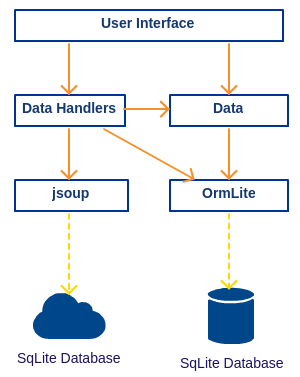
\includegraphics[scale=0.9]{architecture.png}
\caption{Diagram of components}
\end{figure}


\clearpage\pagestyle{Standard}
\section{DETAILED DESCRIPTION OF COMPONENTS, SUBSYSTEMS AND MODULES}
\label{sec:description}

The project will consist of three main components which are User Interface, Middleware, and Data.

\subsection{USER INTERFACE}
\subsubsection{Classification}
User Interface is a package that stores some classes which extend from Java Swing classes. 
\subsubsection{Definition}
The main purpose of User Interface is storing panels and windows to interact with user.
\subsubsection{Responsibilities}
The main responsibility of the component is creating interaction between program and user. \ It 
consists of main window, add course window, delete course window and warning window. \ Main window 
screens schedules, degree summary and configuration of the program with using related panels. \ Add 
course window shows the courses with filter options that can be added to schedule or degree summary. 
\ Delete course window deletes the courses that has been added before. \ Warning window displays 
warnings like class restriction or time conflict for the selected schedule.
\begin{figure}[h]
\centering
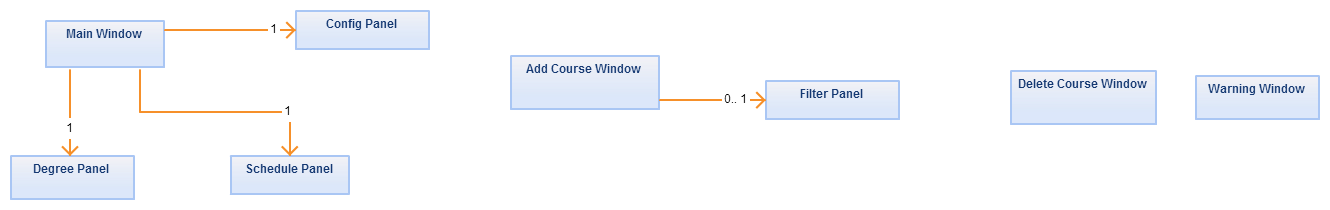
\includegraphics[width=\linewidth]{ui.png}
\caption{Class Diagram of User Interface}
\end{figure}

\subsubsection{Uses/Interaction}
It has a interaction with middleware while getting and setting the schedules and degree summary. \ Degree summary panel and schedule panel creates the windows of add and delete course windows.
\subsubsection{Processing}
Main window contains three panels and shows one of them. \ User can change the panels with the buttons that occur in main window. \ When program opened for the first time, user will see a configuration panel. \ Configuration panel sets the degrees and current term information. Then call the banner parser to get course information from bannerweb. \ When schedule panel is selected, it will pull the data from database connector. \ Schedule panel creates three windows, which are add course window, delete course window and warning window, when it is necessary. \  Degree summary has the same features with schedule panel except that it has no warning window.
\subsection{MIDDLEWARE}
\subsubsection{Classification}
Middleware is a package. It has some classes get data from bannerweb and manipulate before showing them to user.
\subsubsection{Definition}
Middleware connects User Interface and Data to each other as a bridge.
\subsubsection{Responsibilities}
The main responsibility of this component is to manage data for user interface. Banner parser parses  bannerweb for the exact information of courses. \ DB Connector is also other component of middleware which works as bridge that it connects the data to user interface. \ Filter component is looking for the course if it is enable for that filter. \ Course handler component is working for the filtering operation of courses that user specify with the help of filter component. \ It can be course type, time etc..
\begin{figure}[h]
\centering
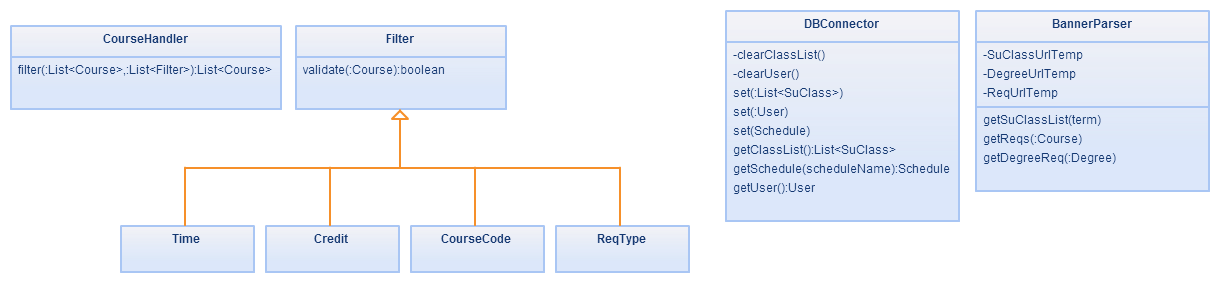
\includegraphics[width=\linewidth]{middleware.png}
\caption{Class Diagram of Middleware}
\end{figure}
\subsubsection{Uses/Interaction}
DB connector interacts with user interface and manipulate data from local database. \ Banner parser talks with configuration panel and pulls the information from bannerweb to send to DB connector. \ Course handler interact with add course window and uses filter classes.
\subsubsection{Processing}
When configuration panel finishes its operation, it calls banner parser. \ When user entered to the schedule panel, degree summary panel or add course window, DB connector called. \ Then they get the releated information by the DB connector. \ When the user adds a new course to his/her schedule, schedule will be updated in database connector. \ When user wants to use any filter, the necessary filter will be occured and the course list will be updated by this information with using course handler.
\subsection{DATA}
\subsubsection{Classification}
Data is a package that stores the information for the application.
\subsubsection{Definition}
Data stores necessary information for the application. 
\subsubsection{Responsibilities}
This package is responsible from storing class, course and user information. \ Also it contains degree requirement. \ It holds schedules that created by the user. \ It is explained also in the figure \ref{fig:datadiagram}.  
\begin{figure}[h]
\centering
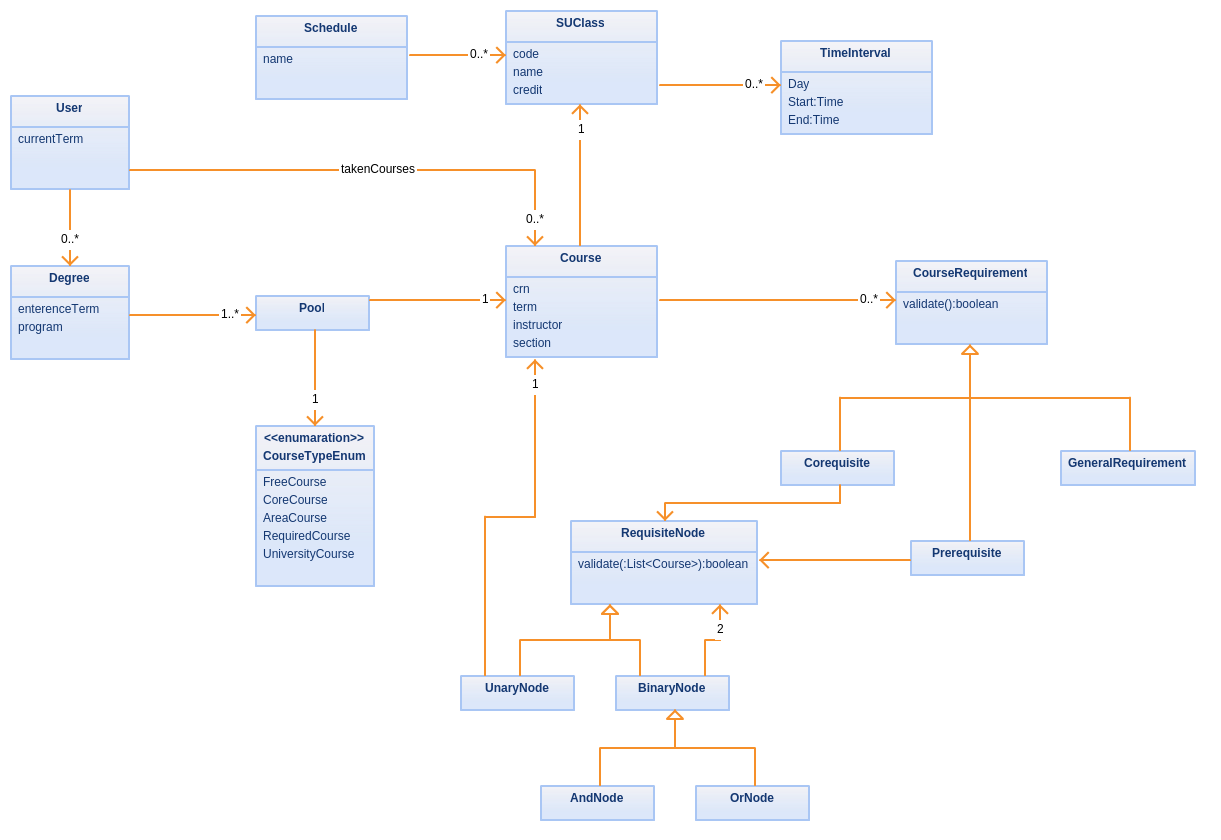
\includegraphics[width=\linewidth]{data.png}
\caption{Class Diagram of Data}
\label{fig:datadiagram}
\end{figure}
\subsubsection{Uses/Interaction}
Course requirement interracts with middleware to create necessary warnings of courses for the user. \ Other classes have no specific methods so there is no other specific interraction to inform. \ This package is mainly used for the capsulation of information.
\subsubsection{Processing}
After user adds a course to the schedule, course requrements of that specific course will be called.\ Then it will return to middleware if a warning exists. \ This process will be repeated for all courses if the warining window pop up.
\end{document}